\documentclass{bredelebeamer}

% Customs:
\usepackage[utf8]{inputenc}
\usepackage{amsmath,amsfonts,amssymb,graphicx}
\usepackage[document]{ragged2e}
\usepackage[Euler]{upgreek}

% Define mathbfit
\DeclareMathAlphabet{\mathbfit}{OML}{cmm}{b}{it}
\DeclareMathAlphabet{\mathbfsf}{\encodingdefault}{\sfdefault}{bx}{n}

\usepackage[backend=biber]{biblatex}
\addbibresource{ref.bib}

% Setting graphics path
\graphicspath{{./rsc/}{./rsc/pdf/}{./rsc/svg/}{./rsc/image/}}

% Define operators
\DeclareMathOperator*{\argmax}{arg\,max}
\DeclareMathOperator*{\argmin}{arg\,min}
\DeclareMathOperator*{\minimize}{Minimize}
\DeclareMathOperator*{\maximize}{Maximize}

% Define textbfit
\makeatletter
\DeclareRobustCommand\bfseriesitshape{
  \not@math@alphabet\itshapebfseries\relax
  \fontseries\bfdefault
  \fontshape\itdefault
  \selectfont
}
\makeatother
\DeclareTextFontCommand{\textbfit}{\bfseriesitshape}

\usefonttheme[onlymath]{serif}

%%%%%%%%%%%%%%%%%%%%%%%%%%%%%%%%%%%%%%%%%%%%%%%% META DATA start

\title[ML Basics]{Linear Models for Regression}
% Titre du diaporama

\subtitle{A self-study metarials for PRML~\cite{bishop:2006:PRML}}
% Sous-titre optionnel

\author{Jisung Lim\inst{1}}
% The \inst {...} command displays the member's affiliation.
% If there are several speakers: Marcel Dupont \inst {1}, Roger Durand
% \inst {2} Simply add another institute on the model below.

\institute[Yonsei]
{
  \inst{1}%
  B.S. Candidate of Industrial Engineering\\
  Yonsei University, South Korea.
}

\date{8th February, 2017}
% Optional. The date, usually the day of the conference.

\subject{Linear Models for Regression, supervised learning.}
% This is used in the pdf metadata

\logo{
  \begin{tikzpicture}
    \pgfmathsetmacro{\myopacity}{0.25}
    \node[opacity=\myopacity] {
      
\includegraphics[scale=0.08]{yonsei_emblem.png}
      
\includegraphics[scale=0.08]{yonsei_logo_text.png}
    };
  \end{tikzpicture}
}

%%%%%%%%%%%%%%%%%%%%%%%%%%%%%%%%%%%%%%%%%%%%%%%% META DATA end

%%%%%%%%%%%%%%%%%%%%%%%%%%%%%%%%%%%%%%%%%%%%%%%% DOCUMENT start

\begin{document}

%%%%%%%%%%%%%%%%%%%%%%%%%%%%%%%%%%%%%%%%%%%%%%%%%%%%%%%%%%% TITLE PAGE

\begin{frame}
  \titlepage
\end{frame}

\printbibliography
%%%%%%%%%%%%%%%%%%%%%%%%%%%%%%%%%%%%%%%%%%%%%%%%%%%%%%%%%%% SUMMARY

\begin{frame}{Summary}
  \tableofcontents
  % Option to add option [pausesections]
\end{frame}

%%%%%%%%%%%%%%%%%%%%%%%%%%%%%%%%%%%%%%%%%%%%%%%%%%%%%%%%%%%%%%%%%%%%%

\section{Introduction}
\subsection{Main concept of linear regression}
\begin{frame}{Main Concept of Linear Regression}
  \begin{block}{The main concept of linear regression}\begin{justify}
    The goal of regression is to predict the value of one or more continuous
    target varaible $\mathit{t}$ (or $\mathbfit{t}$ for more than one variable)
    given the value of a $\mathit{D}$-dimensional vector $\mathbfit{x}$ of input
    variables. Among them, linear regression model is a broad class of functions
    which share the property of being linear functions with respect to the
    adjustable parameters $\theta_j$.
  \end{justify}\end{block}
\end{frame}

\begin{frame}{Linear Models and Regression}
  \begin{justify}
    \textbf{Three componenets of linear regression} \\
    We may see the linear regression as a process
    comprise of three components

    \begin{enumerate}
      \item
      \textbf{N observations} \\
      At first, We retrieve a training data set of $N$ observations $\mathbfit{x}_n$
      together with corresponding target values $t_n$.
      \begin{equation}
        \mathcal{D} = \{(t_1, \mathbfit{x}_1), \ldots, (t_N,\mathbfit{x}_N)\}
      \end{equation}

      \item
      \textbf{Linear Models for Regression} \\
      Given $N$ data set, we will construct linear regression models that comprise
      a broad class of functions which share the property of being linear functions
      with respect to the adjustable parameters $\theta_j$. We may extend the class
      of models by using basis functions $\phi_j(\cdot)$.
      \begin{equation}
        y(\mathbfit{x}, \boldsymbol{\theta}) = \boldsymbol{\theta}^T \boldsymbol{\phi}(\mathbfit{x})
      \end{equation}

      \item
      \textbf{Prediction} \\
      Then, we can construct a function $y(\mathbfit{x})$  which constitute the
      predictions for the target value $t$.
      \begin{equation}
        \hat{t} = y(\mathbfit{x})
      \end{equation}
      or more generally, from a probabilistic perspective we can construct probability
      distribution of $t$ given $\mathbfit{x}$
      \begin{equation}
        p(t|\mathbfit{x})
      \end{equation}
      which expresses our uncertainty about the value of $t$ for each value of
      $\mathbfit{x}$.
    \end{enumerate}
  \end{justify}
\end{frame}

\subsection{Linear models and regression}
\begin{frame}{The Form of Linear Models}
  \begin{justify}
    Linear regression model is a broad class of functions which share the
    property of being linear functions of the adjustable parameters $\theta_j$.
    The form of linear regression models varies from the form of linear combination
    of parameters $\theta_j$ and input variables $x_j$ to the form of linear
    combination of the parameters and a fixed set of nonlinear functions.

    \vspace{1.0\baselineskip}
    Given $\mathbfit{x}={(x_{1}, \ldots, x_{D})}^{\mathit{T}}$, the simplest linear
    model for regression forms:
    \begin{equation}
      f(\mathbfit{x}, \boldsymbol{\theta}) = \theta_0 + \sum_{j=1}^{D} \theta_{j} x_{j} \
    \end{equation}
    which is often simply known as \textit{linear regression}.
    When augmented with other forms of basis function expansion, it can model
    also nonlinear relationships.
    \begin{equation}
      f(\mathbfit{x}, \boldsymbol{\theta}) = \theta_0 + \sum_{j=1}^{M-1} \theta_{k} {\phi_{j} (\mathbfit{x})}
    \end{equation}
    or equivalently, introducing dummy basis function $\phi_{0}(\mathbfit{x}) = 1$ so that
    \begin{equation}
      f(\mathbfit{x}, \boldsymbol{\theta}) = \boldsymbol{\theta}^{\mathit{T}} {\boldsymbol{\phi}(\mathbfit{x})}
    \end{equation}
    the fixed set of nonlinear functions of the input variables $\boldsymbol{\phi}(\mathbfit{x})$
    is known as \textit{basis functions} and $\theta_0$ as \textit{bias parameter}
    which allows for any fixed offset in the data.
  \end{justify}
\end{frame}

\begin{frame}{Linear Models and Basis Function}
  In machine learning approach, we will apply some form of fixed pre-processing
  or feature extraction, to the original data variables.
  \begin{equation}
    \begin{split}
      \textrm{original\ variables}&:\:\mathbfit{x} = {(x_1, \ldots, x_N)}^{T} \\
      \textrm{features}&:\:\boldsymbol{\phi} (\mathbfit{x}) = {(\phi_{0} (\mathbfit{x}), \ldots, \phi_{M-1} (\mathbfit{x}))}^T
    \end{split}
  \end{equation}

  \textbf{Choose of basis function} \\
  \begin{itemize}
    \item Polynomial basis function
          \textrm{(ex)} $\phi_{j} (\mathbfit{x})=x^j$ \\
          Limitation of polynomial basis function is that they are global functions
          of the input variables.
    \item Spline function
          \textrm{(ex)} $\phi_{j} (\mathbfit{x})=f_i (\mathbfit{x})
          \ \textrm{for}\ \mathbfit{x} \in \mathcal{R}_i$ \\
          This can be resolved by dividing the input space up into regions and
          fit a different polynomial $f_i (\mathbfit{x})$ in each region
          $\mathcal{R}_i$.
    \item Gaussian basis function
          \textrm{(ex)} $\phi_{j} (x) = \exp \{ -{(x-\mu^2)}^2 / 2s^2 \}$ \\
          A probabilistic interpretations are not required, and in particular
          the normalization coefficient is unimportant because of the parameters
          $w_j$ which is to be mulitplied to each basis function.
    \item Sigmoid and $\tanh$ basis function
          \textrm{(ex)} $\phi_{j} (x) = \sigma((x-\mu_j) / s)$
          where $\sigma(a)$ is the logistic sigmoid function.
          Since $\tanh(a) = 2\sigma(a) - 1$, generalized linear combination of
          two basis functions can be identically expressed.
    \item Fourier basis function \textrm{(ex)} wavelets.
  \end{itemize}
\end{frame}

\section{Frequentist - linear regression}
\subsection{Prediction by Maximum Likelihood Estimation}
\begin{frame}{Gaussian Noise Assumption}
  \textbf{setting 1.} Additive gaussian noise \\
  Let us assume that the target variable $t$ is given by a deterministic function
  $y(\mathbfit{x}, \mathbfit{w})$ with additive Gaussian noise so that
  \begin{equation}
    t = y(\mathbfit{x}, \mathbfit{w}) + \epsilon
    \quad \textrm{where} \quad \upepsilon \sim \mathcal{N}(\epsilon \:|\: 0, \beta^{-1})
  \end{equation}
  Then, we may express the distribution of target value $t$ as follows
  \begin{equation}
    p(t \:|\: \mathbfit{x},\mathbfit{w},\beta) = \mathcal{N}(\epsilon \:|\: y(\mathbfit{x}, \mathbfit{w}), \beta^{-1})
  \end{equation}

  \vspace{1.0\baselineskip}
  \textbf{setting 2.} Squared loss function \\
  If we set the loss function as a squared loss function as follows
  \begin{equation}
    L(t, y(\mathbfit{x}, \mathbfit{w})) = {\{ t - y(\mathbfit{x}, \mathbfit{w}) \}}^2
  \end{equation}
  and also we can define the expected loss as follows
  \begin{equation}
    \mathbb{E}[L]
    = \iint L(t, y(\mathbfit{x}, \mathbfit{w})) p(t, \mathbfit{x})\, \mathrm{d}t\, \mathrm{d}\mathbf{x}
    = \iint {\{ t - y(\mathbfit{x}, \mathbfit{w}) \}}^2 p(t, \mathbfit{x})\, \mathrm{d}t\, \mathrm{d}\mathbf{x}
  \end{equation}
  Now, to find optimal prediction $y$, set variational derivative of $\mathbb{E}[L]$
  with respect to $y(\mathbfit{x}, \mathbfit{w})$ equals to zero $\delta\mathbb{E}[L] / \delta y = 0$,
  then we get $y^* = \mathbb{E}[t|\mathbfit{x}]$ which will be simply
  \begin{equation}
    y^* = \mathbb{E}[t|\mathbfit{x}]
    = \int tp(t|\mathbfit{x})\, \mathrm{d}t
    = y(\mathbfit{x}, \mathbfit{w})
  \end{equation}
\end{frame}

\begin{frame}{Maximum Likelihood with Basis Function}
  Now, we will construct predictive function $y(t| \mathbfit{x}, \mathbfit{w}, \beta)$
  by using maximum likelihood estimation.

  \vspace{0.5\baselineskip}
  \textbf{$N$ Observations}\\
  At first, Lets consider the input data
  of $N$ observations,
  \begin{equation}
    \mathbf{X} = {(\mathbfit{x}_1, \ldots, \mathbfit{x}_N)}^T
    \quad \textrm{and} \quad
    \mathbfsf{t} = {(t_1, \ldots, t_N)}^T
  \end{equation}

  \textbf{Find likelihood function}\\
  With \textrm{i.i.d.} assumption, we can get the following likelihood function,
  \begin{equation}
    L(\mathbfit{w}) = p(\mathbfsf{t} \:|\: \mathbf{X}, \mathbfit{w}, \beta)
    =\prod_{n=1}^{N} \mathcal{N} (t_n \:|\: \mathbfit{w}^T \boldsymbol{\phi} (\mathbfit{x}_n), \beta^{-1})
  \end{equation}
  taking logarithm of both sides,
  \begin{equation}
    \begin{split}
      \ln L(\mathbfit{w})
      &= \sum_{n=1}^{N} \ln [\mathcal{N} (t_n \:|\: \mathbfit{w}^T \boldsymbol{\phi} (\mathbfit{x}_n), \beta^{-1})] \\
      &= \frac{N}{2}\ln(\beta) - \frac{N}{2}\ln(2\pi)
        -\frac{\beta}{2} \sum_{n=1}^{N} {\{t_n - \mathbfit{w}^T \boldsymbol{\phi} (\mathbfit{x}_n)\}}^2 \\
      &= \frac{N}{2}\ln(\beta) - \frac{N}{2}\ln(2\pi) -\beta E_{D}(\mathbfit{w})
    \end{split}
  \end{equation}
  where $E_{D}(\mathbfit{w})$ is the sum-of-squares error function.
\end{frame}

\begin{frame}{Maximum likelihood with respect to $\mathbfit{w}$}
  \textbf{Maximize $L(\mathbfit{w})$ with respect to $\mathbfit{w}$}\\
  As we've seen before, maximizing the likelihood function $L(\mathbfit{w})$ is
  equivalent to minimizing a sum-of-squares error function $E_{D}(\mathbfit{w})$
  from (16), given the following assumptions
  \begin{equation}
    \mathrm{t} \sim \mathcal{N} (t \:|\: y(\mathbfit{x}, \mathbfit{w}), \beta^{-1})
    \quad \mathrm{with} \quad \mathrm{i.i.d.\ condition}
  \end{equation}
  where $y(\mathbfit{x}, \mathbfit{w}) = \mathbfit{w}^T \boldsymbol{\phi} (\mathbfit{x}_n)$.
  Or we may find same result with the gradient of the log likelihood function,
  \begin{equation}
    \nabla p(\mathbfsf{t} \:|\: \mathbfit{w}, \beta)
    = \sum_{n=1}^{N} [{\{ t_n - \mathbfit{w}^T \boldsymbol{\phi} (\mathbfit{x}_n) \}} {\boldsymbol{\phi} (\mathbfit{x}_n)}^T]
  \end{equation}
  Setting the gradient to zero gives
  \begin{equation}
    0 = \sum_{n=1}^{N} t_n {\boldsymbol{\phi} (\mathbfit{x}_n)}^T
    - \mathbfit{w}^T \left( \sum_{n=1}^{N} \boldsymbol{\phi}(\mathbfit{x}_n){\boldsymbol{\phi}(\mathbfit{x}_n)}^T\right)
  \end{equation}
  Solving for $\mathbfit{w}$, we obtain
  \begin{equation}
    \mathbfit{w}_\mathrm{ML} = {(\boldsymbol{\Phi}^T\boldsymbol{\Phi})}^{-1} \boldsymbol{\Phi}^T \mathbfsf{t}
  \end{equation}
\end{frame}

\begin{frame}{Maximum likelihood with respect to $\beta$}
  \textbf{Maximize $L(\mathbfit{w})$ with respect to $\beta$}\\
  We can also maximize the log likelihood function with respect to the
  noise precision parameter $\beta$, setting derivate of likelihood function
  with respect to $\beta$ equal to zero as follows
  \begin{equation}
    \frac{\partial}{\partial\beta} [p(\mathbfsf{t} \:|\: \mathbfit{w}, \beta)]
    = \frac{N}{2\beta} - E_{D}(\mathbfit{w}) = 0
  \end{equation}
  Then we get,
  \begin{equation}
    \frac{1}{\beta_{\textrm{ML}}} = \frac{2}{N}E_{D}(\mathbfit{w})
     = \frac{1}{N} \sum_{n=1}^{N}{\{t_n - \mathbfit{w}_{\textrm{ML}}^T \boldsymbol{\phi} (\mathbfit{x}_n)\}}^2
  \end{equation}

  \vspace{0.5\baselineskip}
  \textbf{Predictive Function}\\
  Hence, we get predictive function which is given by
  \begin{equation}
    p(t|\mathbfit{x}, \mathbfit{w}_{\mathrm{ML}}, \beta_{\mathrm{ML}})
    = \left({\frac{\beta_{\mathrm{ML}}}{2\pi}}\right)^{1/2}
    \exp{\left[
      -\frac{\beta_{\mathrm{ML}}}{2}
      \left\{
        {t - \mathbfit{w}_{\mathrm{ML}}^T \boldsymbol{\phi}(\mathbfit{x})}
      \right\}^2
    \right]}
  \end{equation}
\end{frame}

\begin{frame}{Normal Equation for the least squares problem}
  \textbf{Normal Equation} \\
  Now consider some conventional terms with the solution (20) for $\mathbfit{w}$
  $$
  \mathbfit{w}_\mathrm{ML} = {(\boldsymbol{\Phi}^T\boldsymbol{\Phi})}^{-1} \boldsymbol{\Phi}^T \mathbfsf{t}
  $$
  which are known as the \textit{normal equations} for the least squares problem.

  \vspace{0.5\baselineskip}
  \textbf{Design Matrix} \\
  Here $\boldsymbol{\Phi}$ is an $N \times M$ matrix, called the \textit{design matrix},
  \begin{equation}
    \boldsymbol{\Phi} =
    \begin{bmatrix}
      {\boldsymbol{\phi} (\mathbfit{x}_1)}^T \\
      \vdots \\
      {\boldsymbol{\phi} (\mathbfit{x}_N)}^T
    \end{bmatrix}
    =
    \begin{bmatrix}
      \boldsymbol{\varphi}_0 &
      \cdots &
      \boldsymbol{\varphi}_{M-1}
    \end{bmatrix}
  \end{equation}
  where
  \begin{equation}
    \begin{split}
      \boldsymbol{\phi} (\mathbfit{x}_n)
      &= {( \phi_0 (\mathbfit{x}_n), \ldots, \phi_{M-1} (\mathbfit{x}_n) )}^T\\
      \boldsymbol{\varphi}_j
      &= { (\phi_j (\mathbfit{x}_1), \ldots, \phi_j (\mathbfit{x}_N) )}^T
    \end{split}
  \end{equation}

  \textbf{Moore-Penrose pseudo-inverse} \\
  And then, the quantity
  \begin{equation}
    \boldsymbol{\Phi}^{\dagger} \equiv {(\boldsymbol{\Phi}^T\boldsymbol{\Phi})}^{-1} \boldsymbol{\Phi}^T
  \end{equation}
  is known as the \textit{Moore-Penrose pseudo-inverse} of the matrix $\boldsymbol{\Phi}$.
\end{frame}

\begin{frame}{The Role of Bias Parameter $w_0$}
  We can get some insight of the role of \textit{Bias Parameter} $w_0$ by solving
  the equation
  \begin{equation}
    \frac{\mathrm{d}}{\mathrm{d}w_0} E_D(\mathbfit{w}) = 0
  \end{equation}

  At first, let us make the bias parameter to be explicit.
  \begin{equation}
    E_{D}(\mathbfit{w}) = \frac{1}{2} \sum_{n=1}^{N} { \left\{ t_n - w_0 - \sum_{j=1}^{M-1} w_j \phi_j (\mathbfit{x}_n)\right\}}^2
  \end{equation}
  Setting the derivative with respect to $w_0$ equal to zero, and solving for
  $w_0$, we obtain
  \begin{equation}
    \begin{split}
      w_0
      &= \frac{1}{N} \sum_{n=1}^{N} t_n - \sum_{j=1}^{M-1} [w_j \frac{1}{N} \sum_{n=1}^{N}\phi_j (\mathbfit{x}_n)] \\
      &= \bar{t} - \sum_{j=1}^{M-1} w_j \bar{\phi}_j
    \end{split}
  \end{equation}
  Thus, the bias $w_0$, as a kind of offset, compensates for the gap between
  the averages of the target values $\bar{t}$ and the linear combination of adaptive
  paramters $w_j$ and the average of the basis functions $\bar{\phi}_j$.
\end{frame}

\subsection{Geometrical Interpretation of Least Squares}
\begin{frame}{Geometry of least squares}
  \textbf{Geometry of least squares}\\
  Let us consider an $N$-dimensional space whose axes are given by the $t_n$,
  so that $\mathbfsf{t} = {(t_1,\ldots,t_N)}^T$ is a specific vector in this space.
  \begin{equation}
    \mathbfsf{t} = {(t_1,\ldots,t_N)}^T \in \mathbb{R}^N
  \end{equation}
  Each basis function $\phi_j (\mathbfit{x}_n)$ may be represented as a vector
  $\boldsymbol{\varphi}_j$ in the same space, when evaluated at the $N$ data points.
  \begin{equation}
    \boldsymbol{\varphi}_j \in \mathbb{R}^N
    \quad \textrm{where} \quad \boldsymbol{\Phi} =
    \begin{bmatrix}
      \boldsymbol{\varphi}_0 & \cdots & \boldsymbol{\varphi}_{M-1}
    \end{bmatrix}
  \end{equation}
  Since $\mathbfsf{y}$ is an arbitrary linear combination of the vector
  $\boldsymbol{\varphi}_j$, it lies on the $M$-dimensional subspace $\mathcal{S}$.
  \begin{equation}
    \mathbfsf{y} = \boldsymbol{\Phi}\mathbfit{w} =
    \begin{bmatrix}
      \boldsymbol{\varphi}_0 & \cdots & \boldsymbol{\varphi}_{M-1}
    \end{bmatrix}
    \:
    \begin{bmatrix}
      w_0 \\ \vdots \\ w_{M-1}
    \end{bmatrix}
    =
    \sum_{j=0}^{M-1} w_j \boldsymbol{\varphi}_j
  \end{equation}
  Hence, intutively, the sum-of-squares error may be understood as the squared
  Euclidean distance between $\mathbfsf{y}$ and $\mathbfsf{t}$. Thus the least-squares
  solution for $\mathbfit{w}$ corresponds to the choice of $\mathbfsf{y}$ that
  lies in subspace $\mathcal{S}$ and that is closest to $\mathbfsf{t}$.
\end{frame}

\subsection{Sequential learning}
\begin{frame}{Sequential learning}
  \begin{justify}
    In cases where the training data set is very large or data is received in a
    stream, a direct solution using the normal equations may not be possible.
    An alternative approach is to use sequential algorithms, also known as on-line
    algorithms. Sequential learning is appropriate for realtime applications in
    which the data observations are arriving in a continuous steam, and predictions
    must be made before all of the data points are seen.

    At first, we will consider tha data points $D_n = \, (n = 1, 2, 3, \ldots)$
    one at a time and then update model parameters after each such consideration.
    \begin{equation}
      \mathcal{D} = \{D_1, \ldots, D_n, \ldots\}
                  = \{(t_1, \mathbfit{x}_1), \ldots, (t_n, \mathbfit{x}_n), \ldots\}
    \end{equation}

    After presentation of $D_n$, the stochastic gradient descent algorithm
    updates the parameter vector $\mathbfit{w}$ using
    \begin{equation}
      \mathbfit{w}^{(\tau+1)} = \mathbfit{w}^{(\tau)} - \eta \nabla E_{n}
    \end{equation}

    The total error function $E$ is the sum of a given error function $E_n$,
    evaluated from the $n$-th data point $D_n$.
    \begin{equation}
      E = \sum_{\forall n} E_n \quad \textrm{where} \quad
      E_n = d(t_n, y(\mathbfit{x}_n))
          = {\{ t_n - \mathbfit{w}^{(\tau)T} \boldsymbol{\phi} (\mathbfit{x}_n) \}}^2
    \end{equation}

    and the algorithms is given as follows, where $\eta$ rerepsents a learning rate.
    \begin{equation}
      \mathbfit{w}^{(\tau+1)} = \mathbfit{w}^{(\tau)} - \eta {\{ t_n - \mathbfit{w}^{(\tau)T} \boldsymbol{\phi} (\mathbfit{x}_n) \}}{\boldsymbol{\phi} (\mathbfit{x}_n)}
    \end{equation}
    This is known as \textit{least-mean-squares} or the \textit{LMS algorithm}.
  \end{justify}
\end{frame}

\subsection{Regularized least squares}
\begin{frame}{Regularized Least Squares}
  Let us adding a regularization term to an error function in order to prevent
  model from over-fitted. The total error function to be minimized takes the form
  \begin{equation}
    E_{D}(\mathbfit{w}) + \lambda E_{W}(\mathbfit{w})
  \end{equation}
  where $\lambda$ is the regulariation coefficient that controls the relative
  importance between the data-dependent error $E_{D}(\mathbfit{w})$ and the
  regularization term $E_{W} (\mathbfit{w})$.

  \vspace{1.0\baselineskip}
  One of the simple forms of regularizer is given by the sum-of-squares of the
  weight vector elements
  \begin{equation}
    E_{W} (\mathbfit{w}) = \frac{1}{2} \mathbfit{w}^T \mathbfit{w}.
  \end{equation}
  If we consider the sum-of-squares error function given by
  \begin{equation}
    E_{D} (\mathbfit{w}) = \frac{1}{2} \sum_{n=1}^N {\{t_n-\mathbfit{w}^T \boldsymbol{\phi} (\mathbfit{x}_n)\}}^2
  \end{equation}
  then the total error function becomes
  \begin{equation}
    E(\mathbfit{w}) = E_{D} (\mathbfit{w}) + E_{W} (\mathbfit{w})
     = \frac{1}{2} \sum_{n=1}^N {\{t_n-\mathbfit{w}^T \boldsymbol{\phi} (\mathbfit{x}_n)\}}^2
     + \frac{\lambda}{2} \mathbfit{w}^T \mathbfit{w}.
  \end{equation}
\end{frame}

\begin{frame}{Other choices of regularizer}
  \textbf{Generalized regularizer}\\
  A more general regularizer is sometimes used, for which the regularized error
  takes the form
  \begin{equation}
    \frac{1}{2} \sum_{n=1}^{N} {\{t_n - \mathbfit{w}^T \boldsymbol{\phi}(\mathbfit{x_n})\}}^2
    + \frac{\lambda}{2} \sum_{j=1}^{M} |w_j|^q
  \end{equation}
  where $q=2$ corresponds to the quadratic regularizer. There are conventional
  terms for linear and quadratic regularizers, respectively, \textit{lasso} and
  \textit{ridge}.

  \vspace{0.5\baselineskip}
  \textbf{Minimizing regularized model and constraind optimization}\\
  For sufficiently large $\lambda = \lambda^*$, we have to minimize regularized
  model (38) to obtain the solution $\mathbfit{w}^*$.
  \begin{equation}
    \minimize_{w_j} \quad
    \sum_{n=1}^{N} {\{t_n - \mathbfit{w}^T \boldsymbol{\phi}(\mathbfit{x_n})\}}^2
    + {\lambda^*} \sum_{j=1}^{M} |w_j|^q
  \end{equation}
  This optimization problem can be seen as a Lagrange multipliers, so that
  it can be represented by constraind optimization problem.
  \begin{equation}
    \begin{split}
      \minimize_{w_j} \quad
      & \sum_{n=1}^{N} {\{t_n - \mathbfit{w}^T \boldsymbol{\phi}(\mathbfit{x_n})\}}^2 \\
      \textrm{subject\ to} \quad
      & \sum_{j=1}^{M} |w_j|^q \leq \eta^*
    \end{split}
  \end{equation}
\end{frame}

\subsection{Multiple outputs}
\begin{frame}{Multiple Outputs}
\end{frame}

\section{Frequentist - model complexity}
\subsection{A frequentist viewpoint of the model complexity}
\begin{frame}{A Frequentist Viewpoint of The Model Complexity}
  \begin{justify}
    \textbf{Model Complexity}\\
    The use of MLE can lead to severe over-fitting if complex models are trained
    using data sets of limited size. For releasing the over-fitting problem, we've
    discussed two approaches:
    \begin{itemize}
      \item limiting the number of basis functions
      \item introducing regularization terms
    \end{itemize}
    But, \textit{the first approach} has side effect of limiting the flexibility
    of the model to capture interesting and important trends in the data. Although,
    \textit{the second approach} reveals the problem of choosing the appropriate
    coefficient $\lambda$.

    \vspace{0.5\baselineskip}
    \textbf{A frequentist viewpoint of the model complexity}\\
    Now we consider the over-fitting issue and model complexity. As we've seen
    before, an over-fitting issue doesn't incur when we marginalize over parameters
    in a Bayesian setting. In the frequentist setting, however, they handle the
    model complexity issue with a special viewpoint, known as the \textit{bias-variance}
    trade-off. At first, we will consider the frequentist view point.
  \end{justify}
\end{frame}

\begin{frame}{Loss Function for Regression}
  \begin{justify}
    In decision theory, we consider the family of functions $y(\mathbfit{x})$ which
    is estimate of the value of $t$, for each input $\mathbfit{x}$. Generally, the
    optimal function $y^* (\mathbfit{x})$ can be chosen by minimizing the loss
    function. And a popular choice of the loss function is the squared loss
    function which is given by
    \begin{equation}
      L(t, y(\mathbfit{x})) = {\{t - y(\mathbfit{x})\}}^2
    \end{equation}
    and the expected loss function is given by
    \begin{equation}
      \begin{split}
        \mathbb{E}[L]
        &= \iint L(t, y(\mathbfit{x})) p(t,\mathbfit{x})\, \mathrm{d}\mathbfit{x}\, \mathrm{d}t \\
        &= \iint {\{t - y(\mathbfit{x})\}}^2 p(t,\mathbfit{x})\, \mathrm{d}\mathbfit{x}\, \mathrm{d}t
      \end{split}
    \end{equation}
    Now we want to find the optimal function $y^* (\mathbfit{x})$, which minimizes
    the expected loss (42), and we can get by setting the variational derivative
    $\delta \mathbb{E}[L] / \delta y(\mathbfit{x})$ equals to zero as follows
    \begin{equation}
      \begin{split}
        &\frac{\delta \mathbb{E}[L]}{\delta y(\mathbfit{x})}
        = 2 \int {\{ y(\mathbfit{x}) - t \}} p(\mathbfit{x}, t) \, \mathrm{d}t = 0 \\
        &\iff
          y(\mathbfit{x}) \int p(\mathbfit{x}, t) \mathrm{d}t
          = \int t p(\mathbfit{x},t) \mathrm{d}t
        \\
        &\iff
          y(\mathbfit{x})
          = \int t \frac{p(\mathbfit{x},t)}{p(\mathbfit{x})} \mathrm{d}t
          = \int t p(t | \mathbfit{x}) \mathrm{d}t
          = \mathbb{E}[t|\mathbfit{x}]
      \end{split}
    \end{equation}
  \end{justify}
\end{frame}

\begin{frame}{Loss Function for Regression (conti\ldots)}
  \begin{justify}
    From the result of (43), for convenience, denote the conditional expectation
    by $h(\mathbfit{x})$, which is given by
    \begin{equation}
      h(\mathbfit{x})
      = \mathbb{E}[t|\mathbfit{x}]
      = \int t p(t | \mathbfit{x}) \mathrm{d}t
    \end{equation}
    Now the expected loss function can be written in the form
    \begin{equation}
      \begin{split}
        \mathbb{E}[L]
        &= \mathbb{E}[{\{t-h(\mathbfit{x})\}}^2] + \mathbb{E}[{\{h(\mathbfit{x})-y(\mathbfit{x})\}}^2]
        + \mathbb{E}[2{\{t-h(\mathbfit{x})\}}{\{h(\mathbfit{x})-y(\mathbfit{x})\}}] \\
        &= \int {\{y(\mathbfit{x}) - h(\mathbfit{x})\}}^2 p(\mathbfit{x}) \, \mathrm{d}\mathbf{x}
        + \iint {\{h(\mathbfit{x}) - t\}}^2 p(\mathbfit{x}, t) \, \mathrm{d}\mathbf{x} \mathrm{d}t
      \end{split}
    \end{equation}
    since
    \begin{equation}
      \begin{split}
        \mathbb{E}[{\{t-h(\mathbfit{x})\}}{\{h(\mathbfit{x})-y(\mathbfit{x})\}}]
        &= \int {\{y(\mathbfit{x})-h(\mathbfit{x})\}} \int {\{h(\mathbfit{x})-t\}} p(\mathbfit{x},t) \, \mathrm{d}t \, \mathrm{d}\mathbfit{x}  \\
        &= \int {\{y(\mathbfit{x})-h(\mathbfit{x})\}} {\left\{h(\mathbfit{x})p(\mathbfit{x}) - \int t p(\mathbfit{x}, t) \mathrm{d}t \right\}} \mathrm{d}\mathbfit{x}\\
        &= 0 \quad \left(\because h(\mathbfit{x}) = \int t p(t|\mathbfit{x}) \mathrm{d}t \right)
      \end{split}
    \end{equation}
  \end{justify}
\end{frame}

\begin{frame}{Loss Function for Regression (conti\ldots)}
  \begin{justify}
    Now consider the equation (45)
    $$
    \mathbb{E}[L]
    = \int {\{y(\mathbfit{x}) - h(\mathbfit{x})\}}^2 p(\mathbfit{x}) \, \mathrm{d}\mathbf{x}
    + \iint {\{h(\mathbfit{x}) - t\}}^2 p(\mathbfit{x}, t) \, \mathrm{d}\mathbf{x} \mathrm{d}t
    $$

    \vspace{0.5\baselineskip}
    \textbf{The second term:} intrinsic, invariant noise\\
    $$
    \mathbb{E}[{\{h(\mathbfit{x})-t\}}^2]
    = \iint {\{h(\mathbfit{x}) - t\}}^2 p(\mathbfit{x}, t) \, \mathrm{d}\mathbf{x} \mathrm{d}t
    $$
    \begin{itemize}
      \item The second term is independent of $y(\mathbfit{x})$.
      \item This quantity arises from the intrinsic noise on the data.
      \item It represents the minimum achievable value of the expected loss.
    \end{itemize}

    \vspace{0.5\baselineskip}
    \textbf{The first term:} Error arose from the choice for the function $y(\mathbfit{x})$\\
    $$
    \mathbb{E}[{\{y(\mathbfit{x})-h(\mathbfit{x})\}}^2]
    = \int {\{y(\mathbfit{x}) - h(\mathbfit{x})\}}^2 p(\mathbfit{x}) \, \mathrm{d}\mathbf{x}
    $$
    \begin{itemize}
      \item The first term depends on our choice for the function $y(\mathbfit{x})$.
      \item We will seek a solution for $y(\mathbfit{x})$ which makes this term a minimum.
      \item Because it is nonnegative, the smallest that we can hope to make this term is zero.
      \item If the data are sufficient enough, we could find the regression function
            $h(\mathbfit{x})$ in any desired degree of accuracy.
    \end{itemize}
  \end{justify}
\end{frame}

\subsection{A bias-variance tradeoffs}
\begin{frame}{Frequentist treatment for modeling the $h(\mathbfit{x})$}
  \begin{justify}
    In a veiwpoint of frequentist, when we model the function $h(\mathbfit{x})$
    using the parametric function $y(\mathbfit{x}, \mathbfit{w})$, since the
    frequentist treatment involves making a point estiamte of $\mathbfit{w}$ based
    on the data set $\mathcal{D}$, they try to understand the uncertainty of
    the estimate as the frequency when we suppose a large number of data sets
    each of which satisfies i.i.d.\ condition.

    \vspace{0.5\baselineskip}
    Let us consider the case where the size of data set is $N$, the number of
    data set is $L$, and each data set is drawn from the distribution $p(t, \mathbfit{x})$
    independently.
    \begin{equation}
      \mathcal{D}^{(l)} = {\{(t_1,\mathbfit{x}_1), \ldots, (t_N,\mathbfit{x}_N)\}}
      \quad \textrm{where} \quad l = 1,\ldots,L \quad \textrm{and} \quad \mathcal{D}^{(l)} \sim p(t,\mathbfit{x})
    \end{equation}
    Then we could run the learning algorithm to obtain a prediction function
    $y(\mathbfit{x};\mathcal{D})$ and then, from the first term of the equation
    (45), the integrand will be given by
    \begin{equation}
      {\{y(\mathbfit{x};\mathcal{D}) - h(\mathbfit{x})\}}^2
      = {\left\{
      \left(y(\mathbfit{x};\mathcal{D}) - \mathbb{E}[y(\mathbfit{x};\mathcal{D})]\right)
      + \left(\mathbb{E}[y(\mathbfit{x};\mathcal{D})] - h(\mathbfit{x})\right)
      \right\}}^2
    \end{equation}
    for any given specific data set $\mathcal{D}$.
  \end{justify}
\end{frame}

\begin{frame}{Frequentist treatment for modeling the $h(\mathbfit{x})$ (conti\ldots)}
  \begin{justify}
    Since the quantity (48) will be dependent on the particular data set $\mathcal{D}$,
    we should take its average over all data sets.
    \begin{equation}
      \begin{split}
        \mathbb{E}[{\{y(\mathbfit{x};\mathcal{D}) - h(\mathbfit{x})\}}^2]
        &= \mathbb{E}\left[{\{
            \left(y(\mathbfit{x};\mathcal{D}) - \mathbb{E}[y(\mathbfit{x};\mathcal{D})]\right)
          + \left(\mathbb{E}[y(\mathbfit{x};\mathcal{D})] - h(\mathbfit{x})\right)
          \}}^2\right] \\
        &= {\left\{\mathbb{E}[y(\mathbfit{x};\mathcal{D})] - h(\mathbfit{x})\right\}}^2
         + \mathbb{E}\left[
           {\left\{y(\mathbfit{x};\mathcal{D}) - \mathbb{E}[y(\mathbfit{x};\mathcal{D})]\right\}}^2
         \right]
      \end{split}
    \end{equation}
    since
    \begin{equation}
      \mathbb{E}[
      \left\{y(\mathbfit{x};\mathcal{D}) - \mathbb{E}[y(\mathbfit{x};\mathcal{D})]\right\}
      \left\{\mathbb{E}[y(\mathbfit{x};\mathcal{D})] - h(\mathbfit{x})\right\}
      ] = 0
    \end{equation}
    Hence, the average quantity over all data sets is given by the form
    \begin{equation}
      \mathbb{E}[{\{y(\mathbfit{x};\mathcal{D}) - h(\mathbfit{x})\}}^2]
      =
      \underbrace{
      {\left\{\mathbb{E}[y(\mathbfit{x};\mathcal{D})] - h(\mathbfit{x})\right\}}^2
      }_{(\textrm{bias})^2}
      +
      \underbrace{
      \mathbb{E}\left[
        {\left\{y(\mathbfit{x};\mathcal{D}) - \mathbb{E}[y(\mathbfit{x};\mathcal{D})]\right\}}^2
      \right]
      }_{\textrm{variance}}
    \end{equation}
    where the equation might be interpreted as the \textbf{bias-variance tradeoffs}.
  \end{justify}
\end{frame}

\begin{frame}{Frequentist treatment for modeling the $h(\mathbfit{x})$ (conti\ldots)}
  \begin{justify}
    Hence, now we can consider the expected loss under the frequentist setting as follows
    \begin{equation}
      \textrm{expected loss} = (\textrm{bias})^2 + \textrm{variance} + \textrm{noise}
    \end{equation}
    \begin{equation}
      \begin{split}
        \mathit{where} \quad (\textrm{bias})^2
        &= \int {\left\{\mathbb{E}[y(\mathbfit{x};\mathcal{D})] - h(\mathbfit{x})\right\}}^2 p(\mathbfit{x}) \mathrm{d}\mathbf{x} \\
        \textrm{variance}
        &= \int {\left\{y(\mathbfit{x};\mathcal{D}) - \mathbb{E}[y(\mathbfit{x};\mathcal{D})]\right\}}^2 p(\mathbfit{x}) \mathrm{d}\mathbf{x} \\
        \textrm{noise}
        &= \iint {\{h(\mathbfit{x}) - t\}}^2 p(t,\mathbfit{x}) \mathrm{d}\mathbfit{x} \mathrm{d}t
      \end{split}
    \end{equation}
    Since we only have finite data sets where $l=1,\ldots,L$, the bias and variance terms are given by
    \begin{equation}
      \begin{split}
        (\textrm{bias})^2
        &= \frac{1}{N} \sum_{n=1}^{N} {\{\bar{y}(\mathbfit{x}_n) - h(\mathbfit{x}_n)\}}^2 \\
        \textrm{variance}
        &= \frac{1}{N} \sum_{n=1}^{N} \frac{1}{L} \sum_{l=1}^{L} {\{y^{(l)}(\mathbfit{x}_n) - \bar{y}(\mathbfit{x}_n)\}}^2 \\
        \mathit{where} &\quad \bar{y}(\mathbfit{x}) = \mathbb{E}[y(\mathbfit{x};\mathcal{D})] = \frac{1}{L} \sum_{l=1}^{L} y^{(l)}(\mathbfit{x})
      \end{split}
    \end{equation}
  \end{justify}
\end{frame}

\begin{frame}{Frequentist treatment for modeling the $h(\mathbfit{x})$ (conti\ldots)}
  \begin{figure}
  \centering
  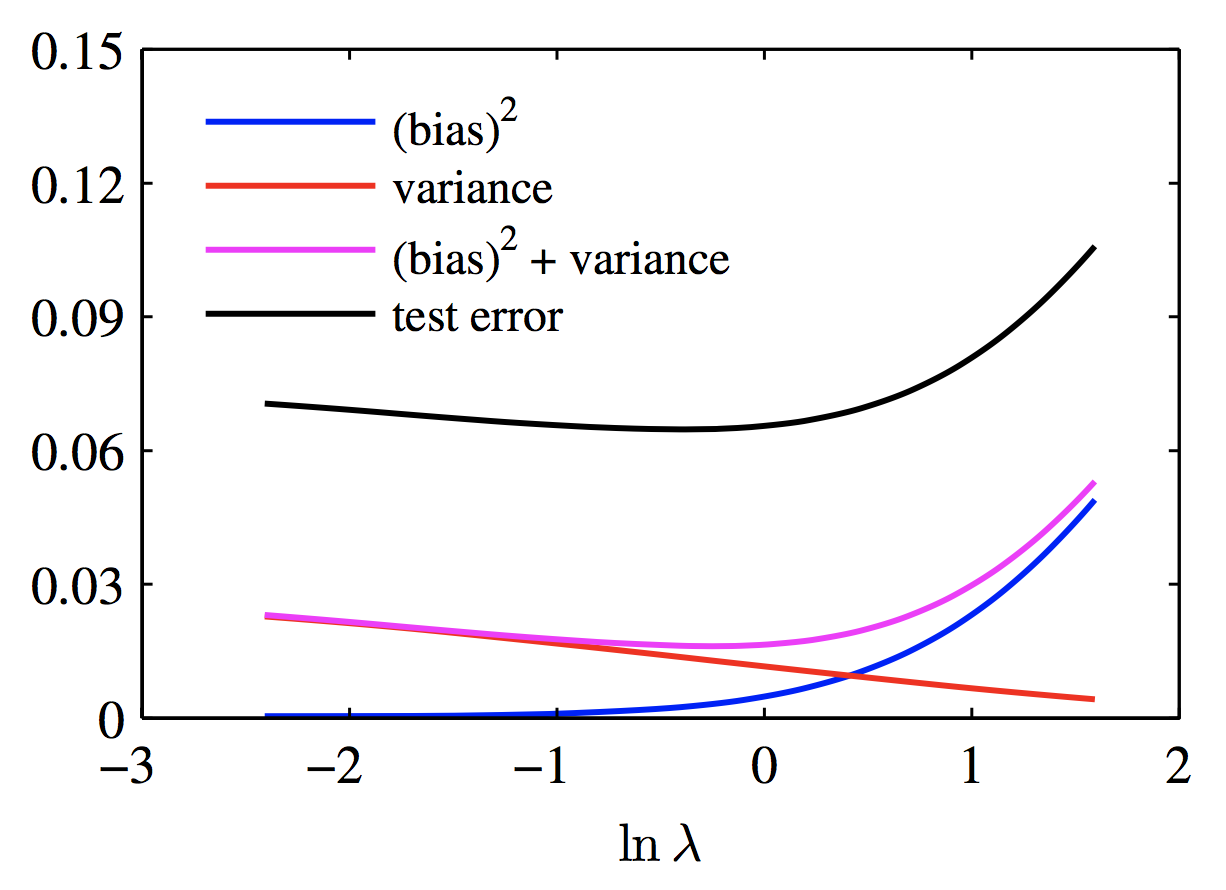
\includegraphics[scale=0.35]{bias_variance_tradeoff.png}
  \caption{
    Loss function for the regularized least-square model.
  }
  \end{figure}
\end{frame}

\section{Bayesian - linear regression}
\subsection{Bayesian approach in linear regression}
\begin{frame}{Bayesian Approach in Linear Regression}
  \textbf{What we've discussed so far} \\
  \begin{itemize}
    \item Effective model complexity; governed by the number of basis function.
    \item Regularizer; governed by the value of the regularization coefficient.
    \item Validation set; too much expensive and wasteful.
  \end{itemize}

  \vspace{0.5\baselineskip}
  \textbf{We, therefore, turn to a Bayesian treatment of linear regression}, which \\
  \begin{itemize}
    \item will avoid the over-fitting problem of Maximum Likelihood approach.
    \item will determine the model complexity automatically, using the training
          data alone.
  \end{itemize}

  \vspace{0.5\baselineskip}
  \textbf{What we will do} \\
  \begin{itemize}
    \item Formulate our knoweledge about the model itself, and prior belief for the
     uncertainty of parameters.
     \begin{equation}
         \textrm{Model}: y(\mathbfit{x},\mathbfit{w}) = \mathbfit{w}^T \boldsymbol{\phi}(\mathbfit{x}) \quad
         \textrm{Parameter}: p(\mathbfit{w}|\alpha)
     \end{equation}
    \item Observe data of $N$ observations
    \begin{equation}
      \mathcal{D} = \{(t_1, \mathbfit{x}_1), \ldots, (t_N, \mathbfit{x}_N)\}
    \end{equation}
    \item Evaluate posterior distribution for the parameters
    \begin{equation}
      p(\mathbfit{w}|\mathcal{D}) \propto L(\mathbfit{w}) p(\mathbfit{w})
    \end{equation}
    \item Make prediction
    \begin{equation}
      p(t|\mathbfsf{t}, \alpha, \beta) = \int p(t|\mathbfit{w},\beta) p(\mathbfit{w}|\mathbfsf{t}, \alpha, \beta) \mathrm{d}\mathbfit{w}
    \end{equation}
  \end{itemize}
\end{frame}

\subsection{Bayesian treatment}
\begin{frame}{Bayesian Treatment}
  First, assume we get the likelihood function from the data which has the form
  \begin{equation}
    \begin{split}
      \textrm{likelihood}:\: p(\mathbfsf{t}|\mathbfit{w})
      = \prod_{n=1}^{N} \mathcal{N}(t_n|\mathbfit{w}^T \boldsymbol{\phi}(\mathbfit{x}_n), \beta^{-1})
      \sim \textrm{Gaussian distribution}
    \end{split}
  \end{equation}
  Since the likelihood function is given by a Gaussian distribution so that the
  conjugate prior and corresponding posterior is also given by a Gaussain
  distribution.
  \begin{equation}
    \textrm{prior}:\: p(\mathbfit{w}) = \mathcal{N}(\mathbfit{w}|\mathbf{m}_0, \mathbf{S}_0)
  \end{equation}
  \begin{equation}
    \textrm{posterior}:\: p(\mathbfit{w|\mathbfsf{t}})
    = \mathcal{N}(\mathbfit{w}|\mathbf{m}_N, \mathbf{S}_N)
  \end{equation}
  where
  \begin{equation}
    \begin{split}
      \mathbf{m}_N &= \mathbf{S}_N (\mathbf{S}_{0}^{-1} \mathbf{m}_0 + \beta \boldsymbol{\Phi}^T \mathbfsf{t})\\
      \mathbf{S}_{N}^{-1} &= \mathbf{S}_{0}^{-1} + \beta \boldsymbol{\Phi}^T \boldsymbol{\Phi}
    \end{split}
  \end{equation}
  Note that,
  \begin{itemize}
    \item $\mathbfit{w}_{\textrm{MAP}} = \mathbf{m}_N$, since the Guassian is
    unimodal distribution whose mode is coincides with its mean.
    \item Also if we chose an infinitely broad prior $\mathbf{S}_0 = \alpha^{-1}\mathbf{I}$
    with $\alpha \rightarrow 0$, the posterior mean $\mathbf{m}_N$ reduces to
    the value $\mathbfit{w}_{\textrm{ML}}$.
    \item Similarly, if $N=0$, the posterior and prior are same.
    \item Furthermore, from the concept of on-line learning, the posterior at
    any stage would become the prior at the next stage.
  \end{itemize}


\end{frame}

\begin{frame}{Bayesian Treatment}
  \textbf{Set the prior}\\
  For simplicity, we will set the prior distribution as follows
  \begin{equation}
    p(\mathbfit{w}|\alpha) = \mathcal{N}(\mathbfit{w}|\mathbf{0}, \alpha^{-1}\mathbf{I})
  \end{equation}

  \textbf{Evaluate the posterior}\\
  We, therefore, get the mean and variance of the posterior given by
  \begin{equation}
    \begin{split}
      \mathbf{m}_N
      &= \beta \mathbf{S}_N \boldsymbol{\Phi}^T \mathbfsf{t}\\
      \mathbf{S}_{N}^{-1}
      &= \alpha \mathbf{I} + \beta \boldsymbol{\Phi}^T \boldsymbol{\Phi}
    \end{split}
  \end{equation}

  \textbf{Maximum a posteriori approach} \\
  Since the posterior is proportional to the product of the prior and the
  likelihood function, the log of the posterior is given by
  \begin{equation}
    \ln p(\mathbfit{w}|\mathbfsf{t})
    = -\frac{\beta}{2} \sum_{n=1}^{N} {\{t_n - \mathbfit{w}^T \boldsymbol{\phi} (\mathbfit{x}_n)\}}^2
      -\frac{\alpha}{2} \mathbfit{w}^T \mathbfit{w} + \textrm{const.}
  \end{equation}
  where maximizing the posterior distribution with respect to $\mathbfit{w}$ is
  equivalent to the minimizing the regularized sum-of-squares error function.
\end{frame}

\begin{frame}{Bayesian Treatment}
  \begin{figure}
  \centering
  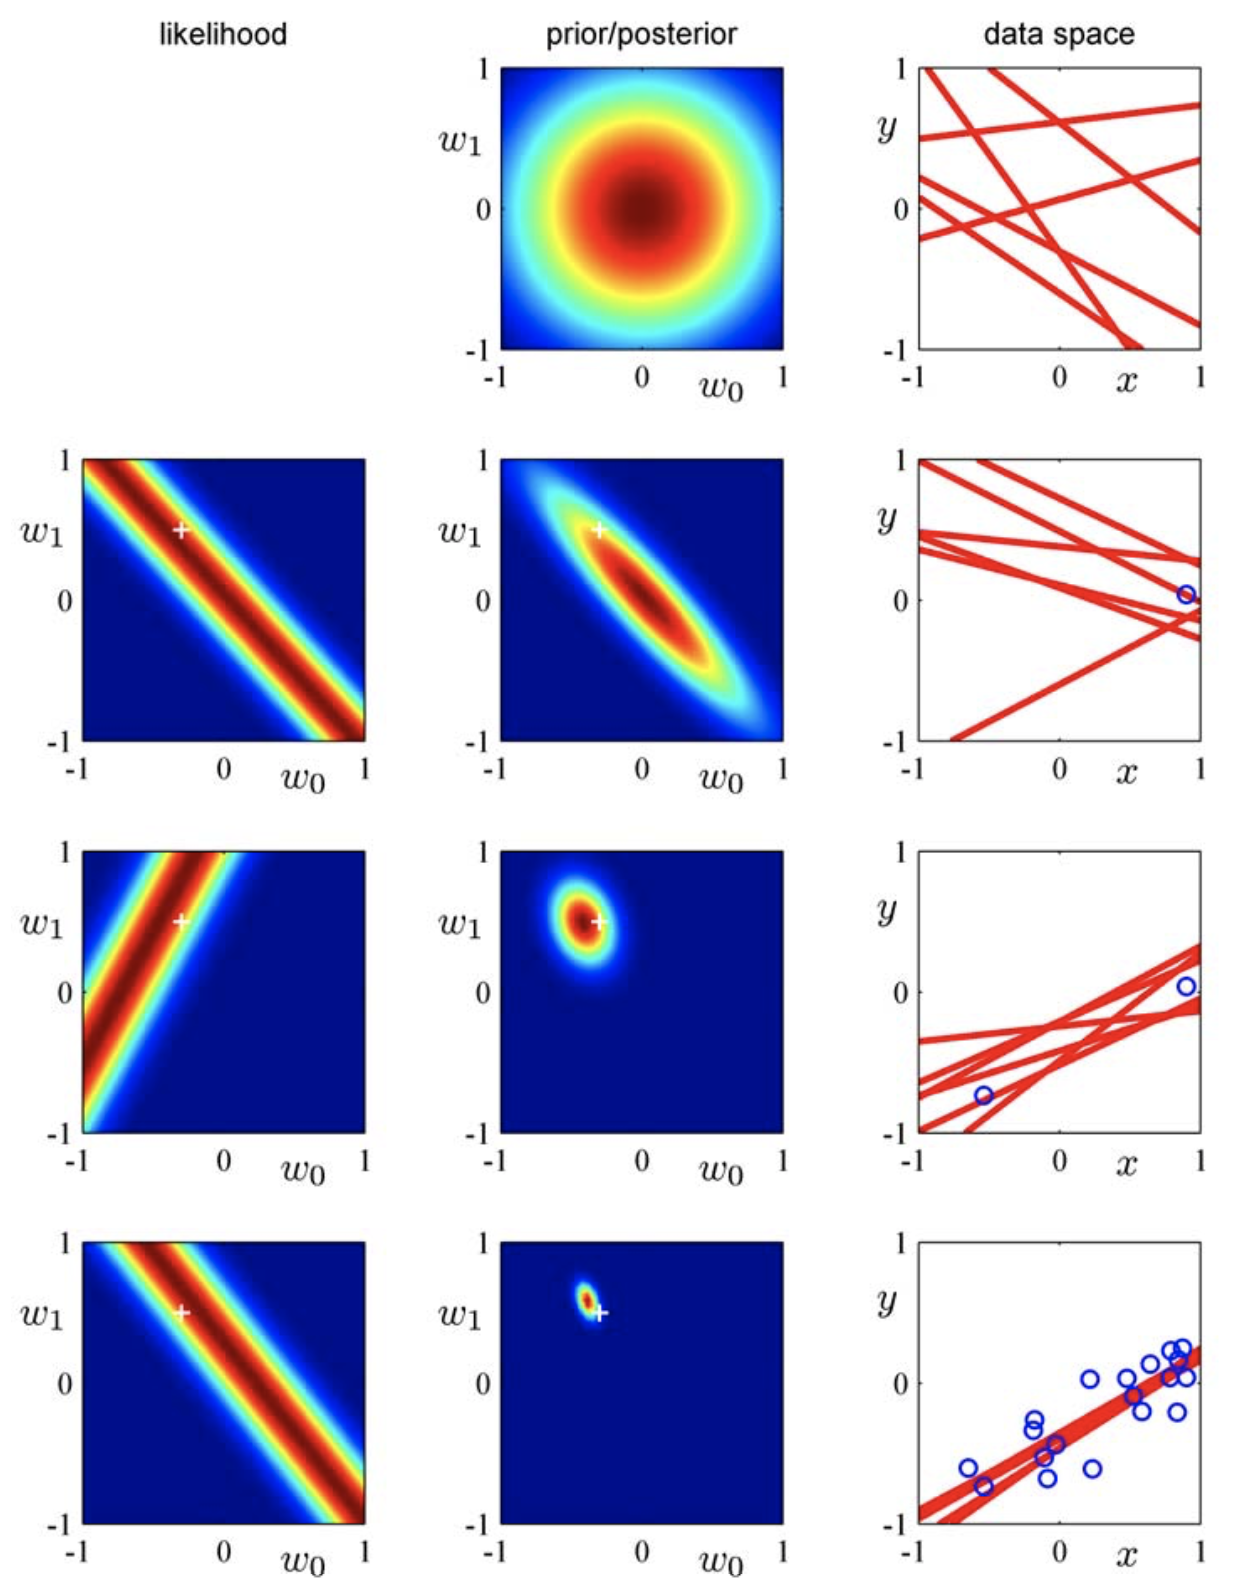
\includegraphics[scale=0.25]{bayesian_treatment.png}
  \caption{
    Illustration of the sequential bayesian treatment.
  }
  \end{figure}
\end{frame}

\begin{frame}{Predictive distribution}
  \begin{justify}
    Indeed, marginalizing multiple solutions with respect to the distribution of
    the parameter $\mathbfit{w}$ lies at the heart of a Bayesian approach. We,
    therefore, get the predictive distribution given by
    \begin{equation}
      \begin{split}
        p(t | \mathbfsf{t}, \alpha, \beta)
        &= \int p(t, \mathbfit{w} | \mathbfsf{t}, \alpha, \beta)\; \mathrm{d}\mathbf{w}\\
        &= \int p(t | \mathbfit{w}, \mathbfsf{t}, \alpha, \beta) p(\mathbfit{w} | \mathbfsf{t}, \alpha, \beta)\; \mathrm{d}\mathbf{w}\\
        &= \int p(t | \mathbfit{w}, \beta) p(\mathbfit{w} | \mathbfsf{t}, \alpha, \beta)\; \mathrm{d}\mathbf{w}
      \end{split}
    \end{equation}
    where the function is not relevant to the parameter $\mathbfit{w}$.
    Since the (62) involves the convolution of two Gaussian distributions, the
    predictive distribution could be the form
    \begin{equation}
      p(t | \mathbfit{x}, \mathbfsf{t}, \alpha, \beta)
      =\mathcal{N} (t | \mathbf{m}_{N}^{T} \boldsymbol{\Phi}(\mathbfit{x}), \sigma_{N}^{2} (\mathbfit{x}))
    \end{equation}
    where
    \begin{equation}
      \sigma_{N}^{2} (\mathbfit{x}) = \frac{1}{\beta} + \boldsymbol{\phi}^T \mathbf{S}_N \boldsymbol{\phi}(\mathbfit{x})
    \end{equation}
    Note that, the first term represents the noise on the data, whereas the
    second term reflects the uncertainty associated with the parameters $\mathbfit{w}$.
    And also, if the size of data set becomes larger, the second term goes to zero.
  \end{justify}
\end{frame}
\begin{frame}{Predictive distribution}
  \begin{figure}
  \centering
  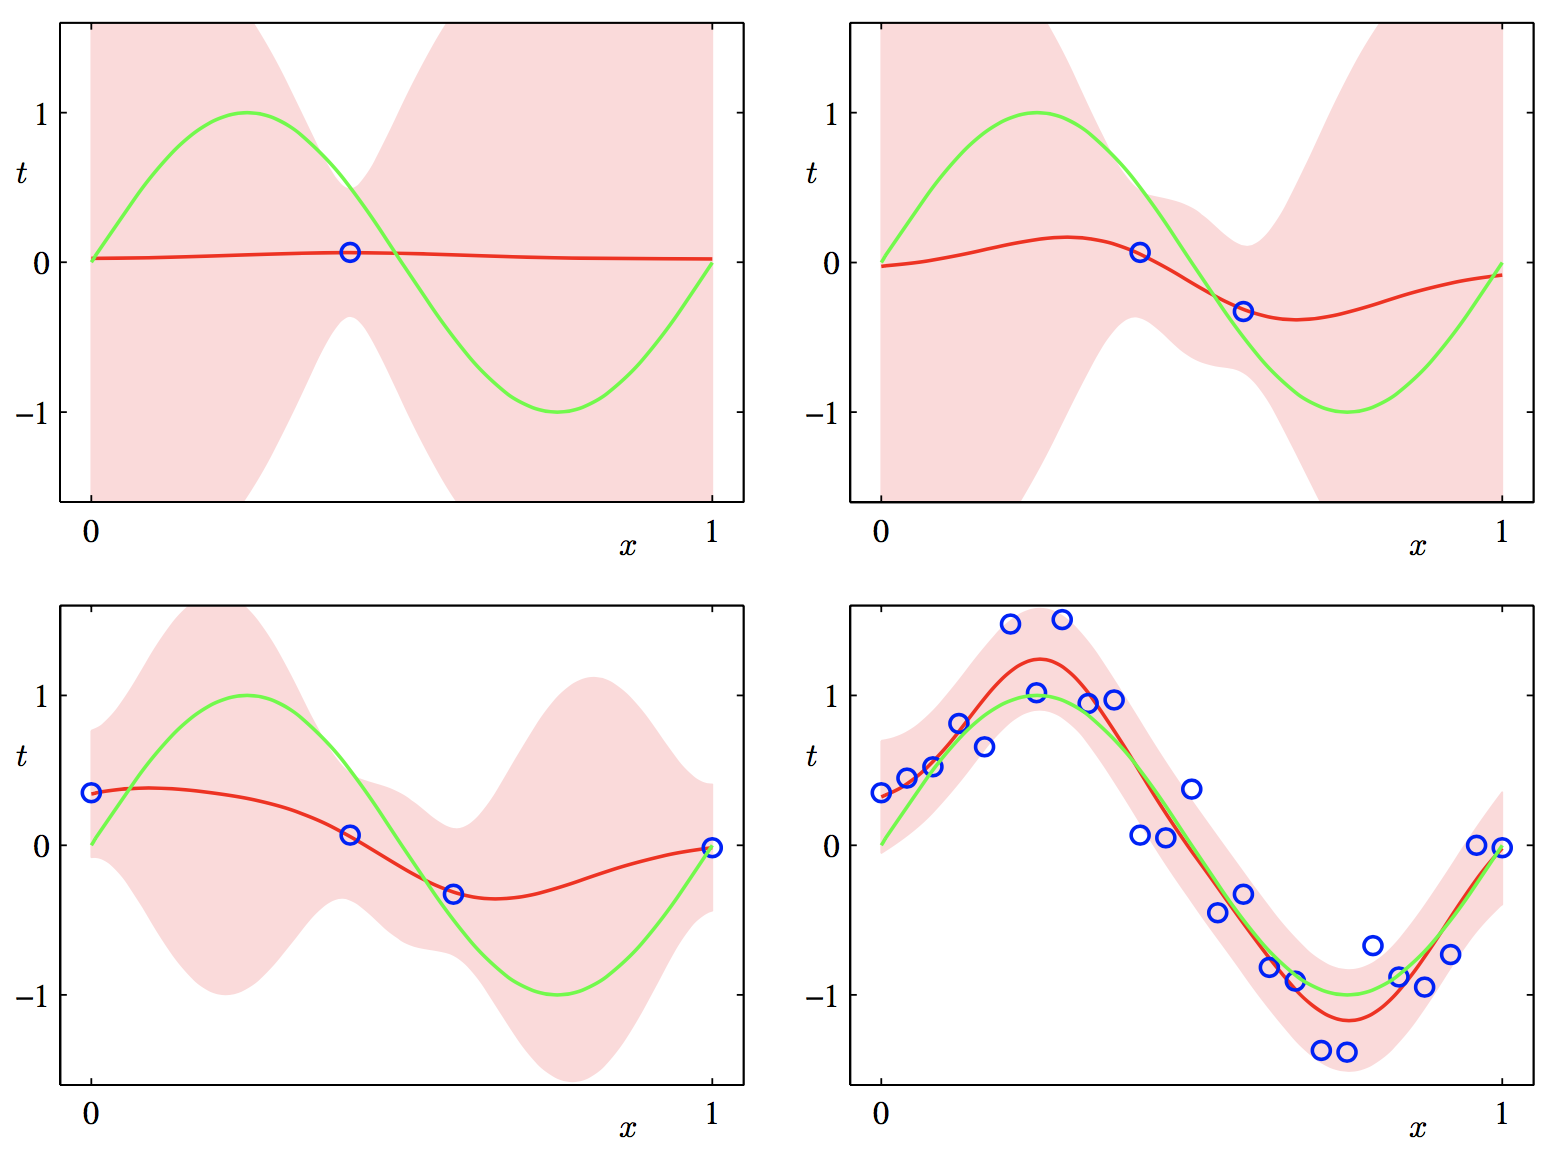
\includegraphics[scale=0.25]{posterior_prediction.png}
  \caption{
    Examples of predictive distributions.
  }
  \end{figure}
\end{frame}

\begin{frame}{Model comparison}
  \begin{figure}
  \centering
  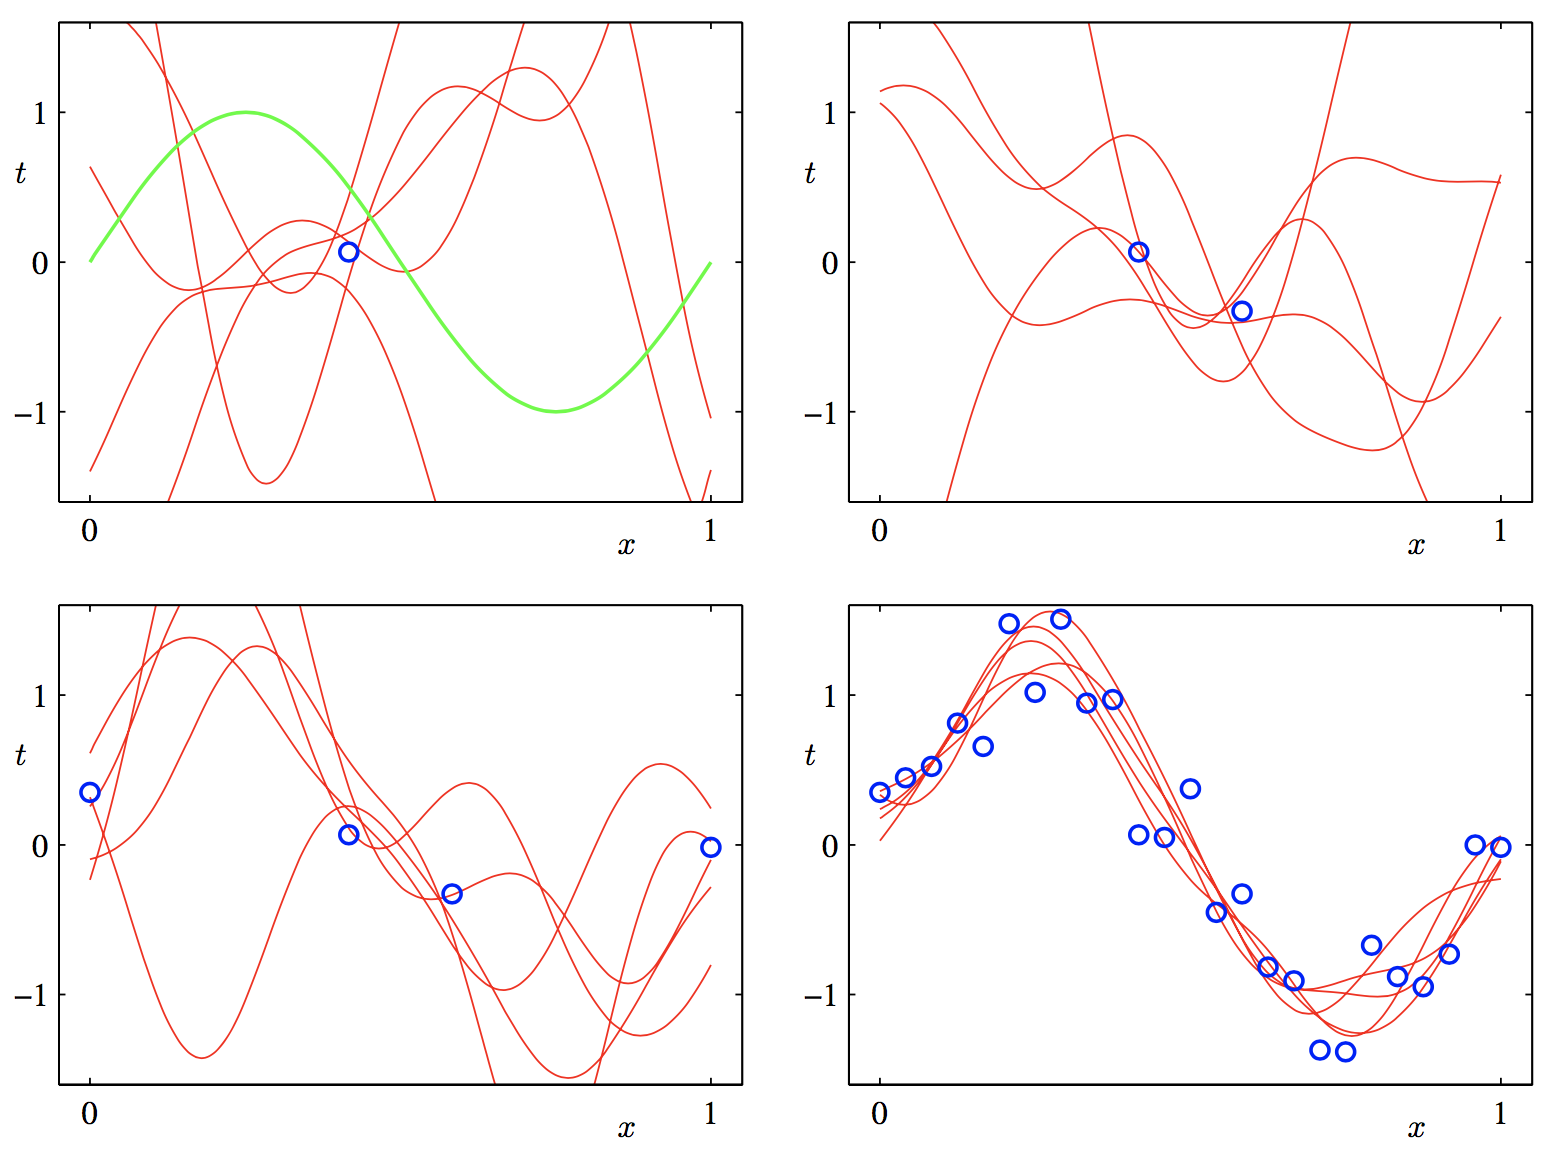
\includegraphics[scale=0.25]{bayesian_model_samples.png}
  \caption{
    Plots of the function $y(x, \mathbfit{w})$ from the posterior distributions.
  }
  \end{figure}
\end{frame}

\subsection{Equivalent kernel}
\begin{frame}{Equivalent Kernel}
  \begin{justify}
    We can see that the predictive mean as a specific model given by
    \begin{equation}
      y(\mathbfit{x}, \mathbf{m}_N)
      = \mathbf{m}_{N}^{T} \boldsymbol{\phi}(\mathbfit{x})
      = \beta {\boldsymbol{\phi}(\mathbfit{x})}^T \mathbf{S}_N \boldsymbol{\Phi}^T \mathbfsf{t}
      = \sum_{n=1}^{N} \beta {\boldsymbol{\phi}(\mathbfit{x})}^T \mathbf{S}_N \boldsymbol{\phi}(\mathbfit{x}_n)t_n
    \end{equation}
    where $\mathbfit{w} = \mathbf{m}_N$. Then, the equation (65) may be interpreted
    as a linear combination of the target variables $t_n$ from training set, so
    that we can write
    \begin{equation}
      y(\mathbfit{x}, \mathbf{m}_N)
      = \sum_{n=1}^{N} k(\mathbfit{x}, \mathbfit{x}_n) t_n
    \end{equation}
    where the function
    \begin{equation}
      k(\mathbfit{x}, \mathbfit{x}')
      = \beta {\boldsymbol{\phi}(\mathbfit{x})}^T \mathbf{S}_N \boldsymbol{\phi}(\mathbfit{x}')
    \end{equation}
    is known as \textit{the smoother matrix} or \textit{the equivalent kernel}.
    And, also \textit{the equivalent kernel} could be obtained by
    \begin{equation}
      \begin{split}
        cov[y(\mathbfit{x}), y(\mathbfit{x}')]
        &= cov[
          {\boldsymbol{\phi}(\mathbfit{x})}^T \mathbfit{w},
          \mathbfit{w}^T\boldsymbol{\phi}(\mathbfit{x}')
        ] \\
        &=
        {\boldsymbol{\phi}(\mathbfit{x})}^T
        \mathbf{S}_N \boldsymbol{\phi}(\mathbfit{x}')
        \\
        &= \beta^{-1} k(\mathbfit{x}, \mathbfit{x}')
      \end{split}
    \end{equation}
    Note that, the predictive mean at nearby points will be highly correlated,
    wheras for more distant pairs of points the correlation will be smaller.
  \end{justify}
\end{frame}

\section{Bayesian - model complexity}
\subsection{A Bayesian viewpoint of the model complexity}
\begin{frame}{A Bayesian Viewpoint of The Model Complexity}
  \textbf{What is model selection?}
  \begin{itemize}
    \item Choosing the value of the hyperparameters.
    \item Choosing a model between alternative models.
  \end{itemize}

  \textbf{How?}
  \begin{itemize}
    \item Frequentist validates their model selection using validation set in
          their Variance-bias framework.
    \item Bayesian use the probabilistic framework to express the uncertainty in
          the choice of model.
  \end{itemize}
\end{frame}

\begin{frame}{Bayesian Model Comparison}
\begin{justify}
  \textbf{Uncertainty of the model} \\
  Now, suppose we wish to compare a set of $L$ models $\{\mathcal{M}_i\}$ and
  suppose that the data $\mathcal{D}$ is generated from one of these models, but
  we are uncertain which one.
  \begin{equation}
    data: \mathcal{D} \quad model: \{\mathcal{M}_i\} \forall i = \{1,\ldots,L\}
  \end{equation}

  \vspace{0.5\baselineskip}
  \textbf{Prior distribution for models} \\
  Each model $\{\mathcal{M}_i\}$ refers to a probability distribution over the
  observed data $\mathcal{D}$. And our uncertainty over models would be expressed
  through a prior probability distribution
  \begin{equation}
    p(\mathcal{M}_i)
  \end{equation}

  \vspace{0.5\baselineskip}
  \textbf{Posterior distribution for models} \\
  Given a training set $\mathcal{D}$, we then wish to evaluate the posterior distibution
  which is calculated by the Bayes' theorem given by
  \begin{equation}
    p(\mathcal{M}_i|\mathcal{D}) \propto p(\mathcal{M}_i) p(\mathcal{D}|\mathcal{M}_i)
  \end{equation}
  The evidence term $p(\mathcal{D}|\mathcal{M}_i)$ also called the marginal likelihood
  function because the parameters $\mathbfit{w}$ are marginalized out.
\end{justify}
\end{frame}

\begin{frame}{Predictive distribution}
  \begin{justify}
    \textbf{Predictive distribution} \\
    Once we know the posterior distribution over models, the predictive distribution
    is given by
    \begin{equation}
      p(t|\mathbfit{x}, \mathcal{D}) = \sum_{i=1}^{L} p(t|\mathbfit{x}, \mathcal{M}_i, \mathcal{D}) p(\mathcal{M}_i|\mathcal{D})
    \end{equation}
    The predictive distribution is marginalized over the space of models.
    \begin{itemize}
      \item $p(t|\mathbfit{x}, \mathcal{M}_i, \mathcal{D})$: Predictive distributions of individual models
      \item $p(\mathcal{M}_i|\mathcal{D})$: Posterior probabilities of those models.
    \end{itemize}

    \vspace{0.5\baselineskip}
    \textbf{Model selection} \\
    A simple approximation to the predictive distribution marginalized over models
    is to use the single, most probable model alone to make predictions. This is
    known as \textit{model selection}.
  \end{justify}
\end{frame}

\begin{frame}{Evidence (Marginal Likelihood)}
  \begin{justify}
    \textbf{Evidence (Marginal Likelihood)} \\
    For a model governed by a set of parameters $\mathbfit{w}$, the model
    evidence is given by
    \begin{equation}
      p(\mathcal{D}|\mathcal{M}_i)
      = \int
        p(\mathcal{D}|\mathbfit{w}, \mathcal{M}_i)
        p(\mathbfit{w}|\mathcal{M}_i)
      \mathrm{d}\mathbfit{w}
    \end{equation}
    \begin{itemize}
      \item $p(\mathcal{D}|\mathbfit{w}, \mathcal{M}_i)$:
      probability of generating the data set $\mathcal{D}$ from a model $\mathcal{M}_i$
      \item $p(\mathbfit{w}|\mathcal{M}_i)$:
      prior distribution for parameters $\mathbfit{w}$
    \end{itemize}

    \vspace{0.5\baselineskip}
    \textbf{Simple Approximation to Evidence} \\
    Now, to get some insight into the model evidence, we approximate the integral.
    At first, let us assume some simplified situation as follows
    \begin{itemize}
      \item The posterior is picked around the most probable value $w_{\textrm{MAP}}$,
      with width $\Delta w_{\textrm{posterior}}$
      \item The prior is flat with width $\Delta w_{\textrm{prior}}$
    \end{itemize}

    Then, we get
    \begin{equation}
      p(\mathcal{D}|\mathcal{M}_i)
      = \int
        p(\mathcal{D}|\mathbfit{w}, \mathcal{M}_i)
        p(\mathbfit{w}|\mathcal{M}_i)
      \mathrm{d}\mathbfit{w}
      \simeq
      p(\mathcal{D}|w_{\textrm{MAP}}) \frac{\Delta w_{\textrm{posterior}}}{\Delta w_{\textrm{prior}}}
    \end{equation}

  \end{justify}
\end{frame}

\begin{frame}{Evidence (Marginal Likelihood)}
  and so taking logs we obtain
  \begin{equation}
    \ln p(\mathcal{D})
    \simeq \ln p(\mathcal{D}|w_{\mathrm{WAP}})
    + \ln \left(
      \frac{\Delta w_{\textrm{posterior}}}{\Delta w_{\textrm{prior}}}
    \right)
  \end{equation}

  With $M$ parameters, all assumed to have the same
  $\Delta w_{\textrm{posterior}} / \Delta w_{\textrm{prior}}$ ratio, we obtain
  \begin{equation}
    \ln p(\mathcal{D})
    \simeq \ln p(\mathcal{D}|\mathbfit{w}_{\mathrm{WAP}})
    + M \ln \left(
      \frac{\Delta w_{\textrm{posterior}}}{\Delta w_{\textrm{prior}}}
    \right)
  \end{equation}

  \begin{itemize}
    \item \textbf{Fitness}:
          $\ln p(\mathcal{D}|\mathbfit{w}_{\mathrm{WAP}})$ \\
          The first term represents the fit to the data given by the most
          probable parameter values. As we increase the complexity of the model,
          it increases because a more complex model is better able to fit the data.
    \item \textbf{Penalty}:
          $M \ln \left(
            \frac{\Delta w_{\textrm{posterior}}}{\Delta w_{\textrm{prior}}}
          \right)$ \\
          The second term represents how much the parameters tuned to the data.
          It penalizes the model according to its complexity. Since it has negative
          values, it decreases as we increase the complexity of the model.
  \end{itemize}
\end{frame}

\begin{frame}{Bayesian Model Comparison}
  \begin{columns}
    \begin{column}{0.5\textwidth}
      \begin{figure}
      \centering
      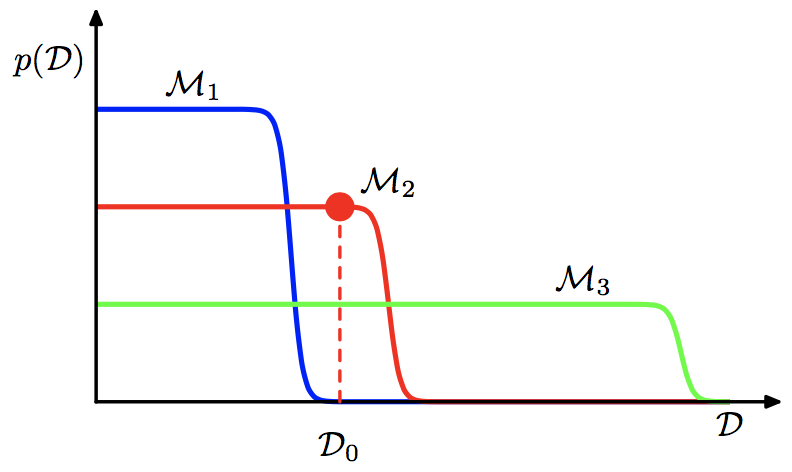
\includegraphics[scale=0.3]{bayesian_model_comparison.png}
      \caption{
        Distribution of possible data set of models.
      }
      \end{figure}
    \end{column}
    \begin{column}{0.5\textwidth}
      \begin{justify}
      How a specific data set $\mathcal{D}$ and its marginal likelihood $p(\mathcal{D})$
      can favour models of intermediate complexity?
      Let's consider the case where we observe a specific data $\mathcal{D}_0$,
      then we may assume three models as follows
      \end{justify}
    \end{column}
  \end{columns}
  \begin{itemize}
    \item Low complexity $\mathcal{M}_1$ \\
          A simple model cannot fit the data well, whereas it assigns larger
          probability than more complex one.
    \item Intermediate complexity $\mathcal{M}_2$ \\
          For specific data $\mathcal{D}_0$ will have the largest probability
          when we choose a model that has intermediate complexity. Simpler one
          can not fit to the data, whereas more complex one can fit to the data
          but it has smaller probabilty.
    \item High complexity $\mathcal{M}_3$ \\
          A complex model spreads its predictive probability, so that it assigns
          relatively small probability.
  \end{itemize}
\end{frame}

\begin{frame}{Model Comparison and Bayes Factor}
  Let consdier two models $\mathcal{M}_1$ and $\mathcal{M}_2$, where the correct
  answer is the model $\mathcal{M}_1$.

  For a given finite data set, it is possible that the Bayes factor flavour
  incorrect answer which is given by

  \begin{equation}
     \frac{p(\mathcal{D}|\mathcal{M}_1)}{p(\mathcal{D}|\mathcal{M}_2)} < 1
  \end{equation}

  However, if we average the Bayes factor over the distrubtion of data sets from
  true model
  \begin{equation}
    \int p(\mathcal{D}|\mathcal{M}_1)
    \ln
      \left(
        \frac{p(\mathcal{D}|\mathcal{M}_1)}{p(\mathcal{D}|\mathcal{M}_2)}
      \right)
    \mathrm{d}\mathcal{D}
    = D_{\textrm{KL}} (\mathcal{M}_1||\mathcal{M}_2) \geq 0
  \end{equation}
  Thus on average the Bayes factor will always favour the correct model.
  For a given
\end{frame}

\subsection{The evidence approximation}
\begin{frame}{The Evidence Approximation}

  \textbf{The fully Bayesian approach} \\
  In the fully Bayesian approach, we would also specify a prior distribution over
  the hyperparameters, such as $\alpha$ and $\beta$, so that they also can be
  marginalized in the Bayesian framework.

  \begin{equation}
    p(t|\mathbfit{x},\mathbfsf{t}) =
    \iiint
    p(t|\mathbfit{x},\mathbfit{w},\beta)
    p(\mathbfit{w}|\mathbfsf{t},\alpha,\beta)
    p(\alpha,\beta|\mathbfsf{t})
    \;
    \mathrm{d}\mathbfit{w}
    \mathrm{d}\alpha
    \mathrm{d}\beta
  \end{equation}

  \begin{itemize}
    \item \textbf{Our model}:
    $p(t|\mathbfit{w}, \beta) = \mathcal{N}(t|y(\mathbfit{x}, \mathbfit{w}), \beta^{-1})$
    \item \textbf{posterior over parameters}:
    $p(\mathbfit{w}|\mathbfsf{t},\alpha,\beta) = \mathcal{N}(\mathbfit{w}|\mathbf{m}_N, \mathbf{S}_N)$
    \item \textbf{posterior over hyperparameters}:
    $p(\alpha, \beta | \mathbfsf{t})$
  \end{itemize}

  \vspace{0.5\baselineskip}
  \textbf{Intractable solution and Evidence approximation} \\
  But the solution above is analytically untractable, so we need to evaluate the
  predictive model by approximating the model distribution. It is also called
  the \textit{evidence approximation}
\end{frame}

\begin{frame}{The Evidence Approximation}
  \textbf{Assumptions for approximation} \\
  Let $p(\alpha, \beta | \mathbfsf{t})$ is sharply peaked around values
  $\hat{\alpha}$ and $\hat{\beta}$, then we get
  \begin{equation}
    p(t|\mathbfsf{t}) \simeq p(t|\mathbfsf{t},\hat{\alpha},\hat{\beta})
    = \int p(t|\mathbfit{w}, \hat{\beta}) p(\mathbfit{w}|\mathbfsf{t},\hat{\alpha},\hat{\beta}) \mathrm{d} \mathbfit{w}
  \end{equation}

  Now, assuming that the prior is relatively flat, from the Bayes' theorem
  \begin{equation}
    p(\alpha, \beta | \mathbfsf{t}) \propto p(\mathbfsf{t}|\alpha,\beta) p (\alpha, \beta)
  \end{equation}

  \textbf{Evidence maximization} \\
  the values of $\hat{\alpha}$ and $\hat{\beta}$ are obtained by maximizing the
  marginal likelihood function which is given by
  \begin{equation}
    p(\mathbfsf{t}|\alpha,\beta) = \int p(\mathbfsf{t}|\mathbfit{w},\beta) p(\mathbfit{w}|\alpha) \mathrm{d}\mathbfit{w}
  \end{equation}
  where
  \begin{equation}
    \begin{split}
      p(\mathbfsf{t}|\mathbfit{w},\beta) &= \prod_{n=1}^{N} \mathcal{N}(\mathbfit{w}^T \boldsymbol{\phi}(\mathbfit{x}_n), \beta^{-1}) \\
      p(\mathbfit{w}|\alpha) &= \mathcal{N}(\mathbfit{w} | \mathbf{0}, \alpha^{-1}\mathbf{I})
    \end{split}
  \end{equation}

  We can re-estimate $\alpha$ and $\beta$ analytically or algorithmically.
  \begin{itemize}
    \item Analytical way: evalute the evidence function, set its derivative equal
          to zero and then obtain re-estimation equations for $\alpha$ and $\beta$
    \item Alternatively, use the technique called the expected maximization
          algorithm.
  \end{itemize}
\end{frame}

\begin{frame}{The Evidence Approximation}
  \textbf{Evaluate the evidence function analytically} \\
  The marginal likelihood is obtained by integrating out parameters
  \begin{equation}
    p(\mathbfsf{t}|\alpha,\beta) = \int p(\mathbfsf{t}|\mathbfit{w},\beta) p(\mathbfit{w}|\alpha) \mathrm{d}\mathbfit{w}
  \end{equation}
  and then we can write the evidence function, by (90), in the form
  \begin{equation}
    p(\mathbfsf{t}|\alpha, \beta)
    =
    {\left(\frac{\beta}{2\pi}\right)}^{N/2}
    {\left(\frac{\alpha}{2\pi}\right)}^{M/2}
    \int \exp \{ - E(\mathbfit{w})\} \mathrm{d}\mathbfit{w}
  \end{equation}
  where
  \begin{equation}
    \begin{split}
      E(\mathbfit{w}) &= \beta E_{D}(\mathbfit{w}) + \alpha E_{W}(\mathbfit{w})
      = \frac{\beta}{2} {||\mathbfsf{t}-\boldsymbol{\Phi}\mathbfit{w}||}^2 + \frac{\alpha}{2} \mathbfit{w}^T \mathbfit{w} \\
      &= E(\mathbf{m}_N) + \frac{1}{2} {(\mathbfit{w} - \mathbf{m}_N)}^T \mathbf{A} (\mathbfit{w} - \mathbf{m}_N)
    \end{split}
  \end{equation}
  where
  \begin{equation}
      \mathbf{A} = \alpha \mathbf{I} + \beta \boldsymbol{\Phi}^T \boldsymbol{\Phi} \quad
      \mathbf{m}_N = \beta \mathbf{A}^{-1} \boldsymbol{\Phi}^T \mathbfsf{t}
  \end{equation}
\end{frame}

\begin{frame}{The Evidence Approximation}
  Hence, we get
  \begin{equation}
    \int \exp{\{ - E(\mathbfit{w}) \}} \; \mathrm{d}\mathbfit{w} = \exp{\{ -E(\mathbf{m}_N) \}} {(2\pi)}^{M/2} |\mathbf{A}|^{-1/2}
  \end{equation}

  Taking logarithm to (91), using (95), the log of marginal likelihood is given by
  \begin{equation}
    \ln p(\mathbfsf{t}|\alpha,\beta)
    = \frac{M}{2}\ln \alpha
    + \frac{N}{2}\ln \beta
    - E(\mathbf{m}_N)
    - \frac{1}{2} \ln |\mathbf{A}|
    - \frac{N}{2} \ln(2\pi)
  \end{equation}
\end{frame}

\begin{frame}{The Evidence Approximation}
  \textbf{Set its derivative equal to zero (WRT $\alpha$)} \\
  Defining the following eigenvector equation
  \begin{equation}
    (\beta\boldsymbol{\Phi}^T \boldsymbol{\Phi}) \mathbfit{u}_i = \lambda_i \mathbfit{u}_i
  \end{equation}

  then $\mathbf{A}$ has eigenvalues $\alpha + \lambda_i$ by
  \begin{equation}
     \mathbf{A} \mathbfit{u}_i = (\alpha + \lambda_i) \mathbfit{u}_i
  \end{equation}

  Evaluate the derivative of the log of the marginal likelihood

  \begin{equation}
    \begin{split}
      \frac{\mathrm{d}}{\mathrm{d}\alpha} \ln p(\mathbfsf{t}|\alpha, \beta)
      &= \frac{\mathrm{d}}{\mathrm{d}\alpha} (\frac{M}{2} \ln{\alpha})
      - \frac{\mathrm{d}}{\mathrm{d}\alpha} (\ln{|\mathbf{A}|})
      - \frac{\mathrm{d}}{\mathrm{d}\alpha} E(\mathbf{m}_N) \\
      &\simeq \frac{M}{2\alpha}
      - \frac{\mathrm{d}}{\mathrm{d} \alpha} \frac{1}{2} \ln{\mathbf{A}}
      - \frac{1}{2} \mathbf{m}_N^T \mathbf{m}_N
    \end{split}
  \end{equation}
  Since
  \begin{equation}
    \frac{\mathrm{d}}{\mathrm{d}\alpha} \ln{|\mathbf{A}|}
    = \frac{\mathrm{d}}{\mathrm{d}\alpha} \ln{\prod_{i=1}^{M} (\lambda_i + \alpha)}
    = \sum_{i=1}^M \frac{1}{\lambda_i + \alpha}
  \end{equation}
  then the stationary point is
  \begin{equation}
    0 = \frac{M}{2\alpha} - \frac{1}{2} \sum_{i=1}^{M} \frac{1}{\lambda_i + \alpha} - \frac{1}{2} \mathbf{m}_N^T\mathbf{m}_N
  \end{equation}
\end{frame}

\begin{frame}{The Evidence Approximation}
  Rearrange the eqaution, then we get
  \begin{equation}
    \alpha \mathbf{m}_N^T \mathbf{m}_N = M - \alpha \sum_{i=1}^{M} \frac{1}{\lambda_i + \alpha} = \gamma
  \end{equation}

  Since $M = \sum_{i=1}^M 1$, then
  \begin{equation}
    \alpha \mathbf{m}_N^T\mathbf{m}_N = \sum_{i=1}^{M} \frac{\lambda_i}{\lambda_i + \alpha} = \gamma
    \quad \textrm{or} \quad
    \alpha = \frac{\gamma}{\mathbf{m}_N^T \mathbf{m}_N}
  \end{equation}

  \textbf{Rearrange sequence} \\
  \begin{enumerate}
    \item Set prior distribution $p(\mathbfit{w})$ over parameters, get $\alpha$, calculate $\gamma$
    \item Evaluate posterior distribution $p(\mathbfit{w}|\mathbfsf{t})$, get $\mathbf{m}_N$
    \item Re-estimate $\alpha$ as $\gamma / \mathbf{m}_N^T \mathbf{m}_N$
  \end{enumerate}
\end{frame}

\begin{frame}{The Evidence Approximation}
  \textbf{Set its derivative equal to zero (WRT $\beta$)} \\
  \begin{equation}
    \frac{\mathrm{d}}{\mathrm{d}\beta} \ln{|\mathbf{A}|}
    = \frac{\mathrm{d}}{\mathrm{d}\beta} \sum_i \ln(\lambda_i + \alpha)
    = \frac{1}{\beta} \sum_i \frac{\lambda_i}{\lambda_i+\alpha} = \frac{\gamma}{\beta}
  \end{equation}
  Then, the stationary point is given by solving the following equation
  \begin{equation}
    0
    = \frac{N}{2\beta}
    - \frac{1}{2} {(\mathbfsf{t}-\boldsymbol{\Phi}\mathbf{m}_N)}^T{(\mathbfsf{t}-\boldsymbol{\Phi}\mathbf{m}_N)}
    - \frac{\gamma}{2\beta}
  \end{equation}

  Therefore, solving the equation, we get
  \begin{equation}
    \beta^{-1}
    = \frac{1}{N-\gamma} \sum_{i=1}^N {\{t_n - \mathbf{m}_N^T \boldsymbol{\phi}(\mathbfit{x}_n)\}}^2
  \end{equation}
\end{frame}

\subsection{An elegant interpretation of $\alpha$ and $\gamma$}
\begin{frame}{An Elegant Interpretation of $\alpha$ and $\gamma$}
  Since, $\boldsymbol{\Phi}^T\boldsymbol{\Phi}$ is positive definitive, the eigenvector
  equation must have postivie eigenvalues $\lambda_i >= 0$. And then we get
  \begin{equation}
    0 \leq \frac{\lambda_i}{\lambda_i + \alpha} \leq 1
  \end{equation}
  And then, we may consider two cases of the value of $\lambda_i$

  \begin{itemize}
    \item ($\lambda_i \gg \alpha$): \\
          The corresponding parameter $w_i$ will be close to its maximum
          likelihood value. The value of $w_i$ is tightly constrained
          by the data. Such parameters are called \textit{well determined}

    \item ($\lambda_i \ll \alpha$): \\
          The corresponding parameter $w_i$ will be close to zero. The value
          of $w_i$ is loosely constrained by the data.
  \end{itemize}

  Now, we can construct a feasible range of $\gamma$ as follows
  \begin{equation}
    0 \leq \gamma = \sum_{i=1}^M \frac{\lambda_i}{\lambda_i + \alpha} \leq M
  \end{equation}

  As the extension of the concept \textit{well determined}, the quantity $\gamma$
  measures the effective total number of well determined parameters.

\end{frame}
%%%%%%%%%%%%%%%%%%%%%%%%%%%%%%%%%%%%%%%%%%%%%%%%%%%%%%%%%%%%%%%%%%%%%
\end{document}
%%%%%%%%%%%%%%%%%%%%%%%%%%%%%%%%%%%%%%%%%%%%%%%% DOCUMENT start
